\section{The Container Storage Interface}
\label{section:background-csi}

The \textit{Container Storage Interface} (CSI) is a standard for exposing
arbitrary block and file storage systems to containerized workloads on container
orchestration systems (COs), such as Kubernetes. Using CSI, third-party storage
providers can write and deploy plugins exposing new storage systems in
Kubernetes without ever having to touch the core Kubernetes code.

\subsection{CSI Driver Architecture}
\label{section:backgroud-csi-plugins-architecture}

Kubernetes interacts with a CSI driver plugin through \textit{Remote Procedure
      Calls} (RPCs). Each CSI driver consists of the following plugins:

\begin{itemize}
      \item
            \textbf{Node Plugin}: A gRPC endpoint serving CSI RPCs that must run
            on the node where the provisioned volume will be published. It
            consists of the CSI driver that implements the CSI \co{Node} service
            and one or more sidecar containers. The kubelet of every node is
            responsible for issuing the CSI Node service calls. The kubelet
            issues the calls to the Node service of the driver through a UNIX
            domain socket on the host shared via a \co{HostPath} volume. The
            node plugin has direct access to the host for making block devices
            and filesystem mounts available to the kubelet.
      \item
            \textbf{Controller Plugin}: A gRPC endpoint serving CSI RPCs that
            may run on any node of the cluster. It consists of the CSI driver
            that implements the CSI \co{Controller} service and one or more
            sidecar containers. These controller sidecar containers typically
            interact with Kubernetes objects and make calls to the driver's CSI
            Controller service by sharing a UNIX domain socket through an
            \co{emptyDir} volume between the sidecars and CSI driver. It
            generally does not need direct access to the host.
\end{itemize}

%TODO: Scheme drivers

\paragraph*{The Google Remote Procedure Call}

We mentioned earlier that a container orchestrator  interacts with the driver
through RPCs. The most widely used RPCs are \textit{Google Remote Procedure
      Calls} (gRPC). gRPC is an open-source, high-performance Remote Procedure Call
(RPC) framework that can run in any environment. It uses HTTP/2 for transport,
Protocol Buffers as the interface description language, and provides
authentication, bidirectional streaming and flow control features, blocking or
non-blocking bindings, and cancellation and timeouts. It generates
cross-platform client and server bindings for many languages. gRPC clients and
servers can run and talk to each other in various environments and can be
written in any of gRPC’s supported languages.

\begin{figure}[ht]
      \centering
      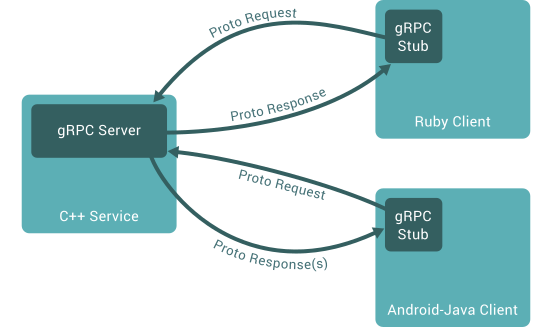
\includegraphics[width=0.6\textwidth]{resources/grpc.png}
      \caption{The architecture of gRPC}
\end{figure}


\subsection{The CSI Remote Procedure Calls}

\begin{figure}[ht]
      \centering
      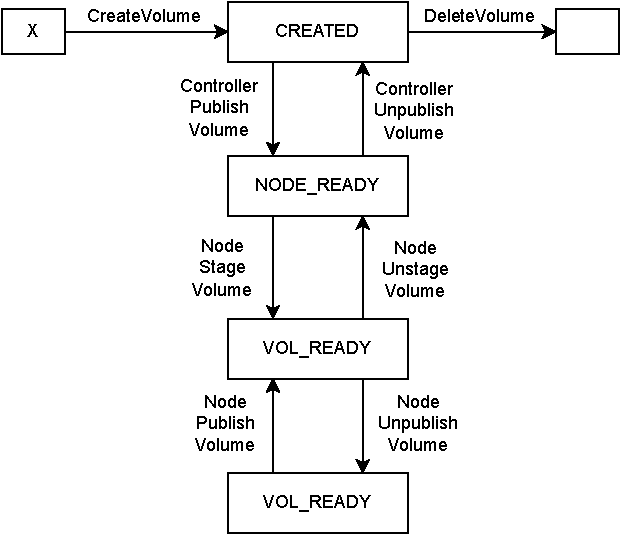
\includegraphics[width=0.7\textwidth]{resources/csi-states.pdf}
      \caption{The lifecycle of a dynamically provisioned volume, from creation
            to destruction.}
      \label{figure:csi-calls}
\end{figure}

The Container Storage Interface defines the RPCs a container orchestrator uses
in order to interact with the storage driver. Each of the RPCs is an idempotent
operation. The order the calls can be issued is show in Figure
\ref{figure:csi-calls}. The list of available RPCs is the following:

\begin{itemize}

      \item{\co{CreateVolume}}: The external provisioner issues this RPC to the
            CSI Controller service, asking it to provision a new volume on
            behalf of a user. If the plugin is unable to complete the
            \co{CreateVolume} call successfully, it must return a non-OK gRPC
            code in the gRPC status.

            Of particular interest in the context of the thesis is the
            \co{RESOURCE\_EXHAUSTED} code; If the controller plugin responds
            with this code, it indicates that it cannot provision the requested
            volume with the specified topology constraints, possibly due to
            insufficient storage capacity.

      \item{\co{ControllerPublishVolume}}: The external attacher issues
            this RPC to the CSI Controller service when Kubernetes wants to
            place a workload that uses the (already provisioned) volume onto a
            node. The plugin should perform the necessary work to make the
            volume available on the given node.

      \item{\co{NodeStageVolume}}:  The kubelet issues this RPC to the  CSI Node
            service when the volume is to be used by the first Pod on the node.
            It should be issued only after \co{NodePublishVolume} has succeeded.
            It is essentially used to format the volume and mount it on a
            staging directory on the node.

      \item{\co{NodePublishVolume}}: The  kubelet issues this RPC to the  CSI
            Node service when a Pod starts to run on a node. It essentially
            mounts the volume to the directory of the Pod.

      \item{\co{NodeUnpublishVolume}}: The kubelet issue this RPC to the CSI
            Node service to undo the work done by the corresponding
            \co{NodePublishVolume}. It essentially unmounts the volume from the
            directory of the Pod.

      \item{\co{NodeUnstageVolume}}: The kubelet issues the RPC to the CSI Node
            service to undo the work by the corresponding \co{NodeStageVolume}.
            It essentially unmounts the volume from the staging directory of the
            node.

      \item{\co{ControllerUnpublishVolume}}: The external attacher issues this
            RPC to the CSI Controller service to perform the work necessary for
            making the volume ready to be consumed by a different node. It
            essentially undoes any work done by the
            \co{ControllerPublishVolume}.

      \item{\co{DeleteVolume}}: The external provisioner issues this RPC to the
            CSI Controller service to deprovision a volume. It is the reverse
            operation of the \co{CreateVolume}.

\end{itemize}


\subsection{Kubernetes CSI Sidecars}
The Kubernetes CSI sidecars containers are a set of standard containers that aim
to simplify the development and deployment of CSI drivers on Kubernetes. These
containers contain common logic to watch the Kubernetes API, trigger appropriate
operations against the \textit{CSI driver} container, and update the Kubernetes
API as appropriate. The containers are intended to be bundled with third-party
CSI driver containers and deployed together as Pods.



\subsubsection{CSI External Provisioner}
\label{csi-external-provisioner}
\label{section:provisioner}

The CSI external provisioner is a sidecar container that watches the Kubernetes
API server for \texttt{PersistentVolumeClaim} objects. If a PVC requests for
dynamic provisioning of a volume and has the selected node annotation
\footnote{Selected node annotation: \co{volume.kubernetes.io/selected-node:
            <node-name>}}, the external provisioner issues a \co{CreateVolume} RPC against
the CSI Controller service to provision a new volume accessible from the
selected node. Suppose the Controller service responds with a
\co{ResourceExhausted} status code. In that case, the external provisioner will
remove the selected node annotation from the PVC, to signal back to the
scheduler that the provisioning of the volume has failed, and it shall retry the
scheduling. Once the external provisioner successfully provisions the volume, it
creates a Kubernetes \texttt{PersistentVolume} object to represent the volume
and binds it to the PVC.

The deletion of a \texttt{PersistentVolumeClaim} object bound to a
\texttt{PersistentVolume} corresponding to this driver with a \texttt{delete}
reclaim policy causes the external provisioner to trigger a
\texttt{DeleteVolume} operation against the CSI Controller service to delete the
volume. Once the volume is successfully deleted, the sidecar container deletes
the \texttt{PersistentVolume} object representing the volume.

\subsubsection{CSI External Attacher}

The CSI external attacher is a sidecar container that watches the Kubernetes API
server for \texttt{VolumeAttachment} objects and triggers
\co{ControllerPublishVolume} and \co{ControllerUnpublishVolume} operations
against a CSI endpoint.


\subsubsection{CSI Node Driver Registrar}

The CSI node driver registrar is a sidecar container that fetches driver
information  by issuing a \texttt{NodeGetInfo}) to the CSI Node service and
registers the driver with the kubelet on that node.  The registration is
necessary because the kubelet is responsible for issuing CSI \co{NodeGetInfo},
\co{NodeStageVolume}, \co{NodePublishVolume} calls. By registering the CSI
driver, the kubelet learns which Unix domain socket to issue the CSI calls on.